\documentclass{article}
\usepackage[utf8]{inputenc}
\usepackage[polish]{babel}
\usepackage{polski}
\usepackage{enumerate}
\usepackage{natbib}
\usepackage{graphicx}
\usepackage{geometry}
\usepackage{float}

\newgeometry{tmargin=2.5cm, bmargin=2.5cm, lmargin=2.5cm, rmargin=2.5cm}

\makeatletter
\newcommand{\linia}{\rule{\linewidth}{0.4mm}}
\renewcommand{\maketitle}{\begin{titlepage}
    \vspace*{1cm}
    \begin{center}
    Politechnika Wrocławska\\
    AiR ARR\\
 Projekt zespołowy
    \end{center}
      \vspace{3cm}
    \begin{center}

     \LARGE \textsc {\@title}
         \end{center}
     \vspace{1cm}

    \begin{center}
    \textit{ Autorzy:}\\
   \textit{\@author}
     \end{center}
      \vspace{1cm}

     \begin{center}

    Prowadzący:
  dr inż. Krzysztof Arent %dorobić inż mgr itd
    \end{center}

    \vspace*{\stretch{6}}
    \begin{center}
    \@date
    \end{center}
  \end{titlepage}
}
\makeatother
\author{Beata Berajter\\
Dawid Brząkała\\
Dorota Gidel\\
Katarzyna Wądrzyk\\
Ada Weiss\\
Małgorzata Witka-Jeżewska\\
 }%wpisać indeks
\title{SensGlove}

\begin{document}

\maketitle
\newpage
\tableofcontents
\newpage


\section{Wymagania użytkownika}
Użytkownik powinien mieć możliwość założenia sprzętu, to znaczy rękawiczki sensorycznej oraz czujników miopotencjałów, oraz uruchomienia programu służącego do odbioru ich. Wtedy, po poprawnym podłączeniu się, użytkownik powinien mieć możliwość podglądu w czasie rzeczywistym wykonywanych ruchów. W przypadku poprawnego działania każdego z czujników użytkownik powinien mieć możliwość utworzenia odpowiedniego folderu i zapisania do niego wyników odczytów z czujników od momentu wciśnięcia przycisku START do zdefiniowanej wcześniej długości czasu. Użytkownik powinien mieć możliwość wykonania i zapisu dowolnej ilości pomiarów oraz stworzenie dowolnej ilości folderów oznaczających kolejne gesty.

\section{Kryteria ewaluacji}
Komponenty powinny działać każde z osobna oraz współdziałać jako kompletne stanowisko do pobierania sygnałów i biosygnałów. 


\section{Specyfikacja funkcjonalności}
\section{Rozpoznanie możliwości wykonania bazy sprzętowo-programowej}

\subsection{Projekt oparty na płytce deweloperskiej STM32F3Discovery}
ZALETY:\\
\begin{enumerate}
    \item 
    \item 
\end{enumerate}
WADY:\\
\begin{enumerate}
    \item 
    \item 
\end{enumerate}
\subsection{Projekt oparty na dostępnej już karcie }
ZALETY:\\
\begin{enumerate}
    \item 
    \item 
\end{enumerate}
WADY:\\
\begin{enumerate}
    \item 
    \item 
\end{enumerate}
\subsection{Projekt oparty na karcie }
ZALETY:\\
\begin{enumerate}
    \item 
    \item 
\end{enumerate}
WADY:\\
\begin{enumerate}
    \item 
    \item 
\end{enumerate}
\section{Podział na komponenty, architektura i kryteria ewaluacji komponentów}
\subsection{Rękawiczka sensoryczna}
% potrzebny sprzęt i elementy, konkretne  czujniki, ich liczba, ich dokumentacja, cena (pamiętajcie o wyborze rękawiczki!), czas na uzyskanie ich
% wstępna koncepcja rozmieszczenia elementów, opis słowno-muzyczny
% schematy ideowe, sposób podłączania, ilość wejść i wyjść, zakresy działania z dołączonej dokumentacji
% poszczególne zadania, jakie trzeba wykonać i kto je zrobi, najlepiej przypisane do jednej osoby
% sposób testowania, czy działa, rozpisanie na poszczególne kryteria
% napisanie co będzie oznaczać wykonania zadania poprawnie
\subsection{Interfejs sprzętowy}
% potrzebny sprzęt i elementy, ich liczba, ich dokumentacja, cena, czas na otrzymanie ich
% wstępna koncepcja rozmieszczenia elementów, opis słowno-muzyczny
% schematy ideowe, sposób podłączania, ilość wejść i wyjść, zakresy działania z dołączonej dokumentacji
% potrzebne biblioteki
% BARDZO WAŻNE, kryterium sprawdzające, czy odczyty są zsynchronizowane!
% suma kontrolna
% poszczególne zadania, jakie trzeba wykonać i kto je zrobi, najlepiej przypisane do jednej osoby
% propozycja wysyłania danych
% sposób testowania, czy działa, rozpisanie na poszczególne kryteria
% napisanie co będzie oznaczać wykonania zadania poprawnie
Osaba przydzielona do zadania: Dawid Brząkała \\
Interfejs będzie miał za zadanie odczyt wartości z czujników zgięcia i nacisku z rękawiczki oraz czujników biopotencjałów i przesyłał je w odpowiednim formacie do komputera poprzez kabel USB i wirtualny port COM. Sygnały z czujników zostaną wzmocnione przez układ ze wzmacniaczami operacyjnymi, który również zadba o to, aby wartości sygnałów wyjściowych mieściły się w zakresie pracy przetwornika ADC mikrokontrolera (0 - 3.3V). Zasilanie układu pochodzić będzie ze złącza USB.
\subsubsection{Schemat ideowy}
% plik "schemat ideowy interfejsu.png" nie wiem jak się wstawia obrazki
\begin{figure}[ht!]
\centering
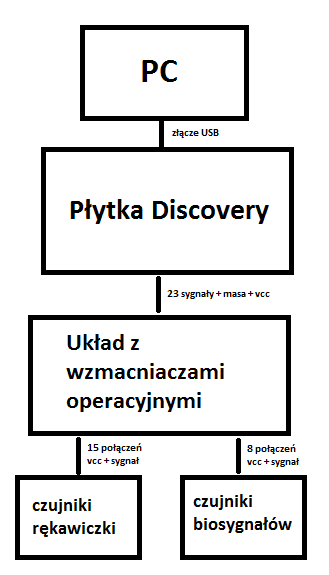
\includegraphics[width=6cm]{schemat_ideowy_interfejsu.png}
\label{fig:interfejs}
\caption {Schemat ideowy interfejsu sprzętowego}

\end{figure}


\subsubsection{Potrzebne elementy}

Lista elementów wraz z przewidywanymi kosztami została przedstawiona w tabeli \ref{tab:interfejs}.
\begin{table}[ht!]
\centering
\caption{ Lista potrzebnych elementów}

\begin{tabular}{|r|l|l|} \hline

element & ilosc & cena\\ \hline
rezystory 10kOhm & 20 & 0.60zł/10szt \\ 
listwa kołkowa 1x40 pin & 1 & 0.69zł/szt \\
listwa kołkowa 2x40 pin & 1 & 1.00zł/szt \\
wzmacniacz operacyjny TL084 & 6 & 8,34zł/szt \\
dioda zenera 3V3 & 24 & 0.12zł/szt \\
STM32F3 - DISCOVERY - Cortex-M4F & 1 & 102.90zł/szt \\
laminat światłoczuły 100x160x1.5mm dwustronny + & 1 & 15.00zł/szt \\\hline % jeśli wytrawiamy sami, jak będziemy zamawiać będzie trzeba zmienić
razem & & 131.41zł \\\hline
\end{tabular}
\label{tab:interfejs}
\end{table}


\subsubsection{Kryteria ewaluacji}
Aby sprawdzić poprawność odczytu sygnałów przez przetworniki ADC czujniki będą symulowane poprzez potencjometry, a uzyskane wyniki przesłane do komputera. Poprawność samej transmisji sprawdzona zostanie poprzez wysyłanie zaprogramowanych wcześniej przykładowych wiadomości i odczytywanie ich w komputerze poprzez program do monitownia portów COM.
\subsection{Program do akwizycji danych}
Osoby przydzielone do zadania: Ada Weiss, Małgorzata Witka-Jeżewska\\
Zadaniem programu będzie odczyt danych przesyłanych z mikrokontrolera z portu USB komputera. Użytkownik po uruchomieniu programu będzie miał możliwoć rozpoczęcia procesu akwizycji danych. Dane będą wczytywane przez okreslony czas (prawdopodobnie 2s jak w dotychczasowych badaniach niosygnałów z przedramienia, co pozwoliłoby na synchronizację tych pomiarów) odszyfrowywane i przesyłane do programu do tworzenia wizualizacji rękawiczki i danych z sensorów z wykorzystaniem socketów. Dodatkowo program będzie umożliwiał użytkownikowi wybór typu ruchu który jest obecnie wykonywany. Każdorazowo po wykonanym pomiarze użytkownik będzie musiał zdecydować czy dany pomiar zapisać czy go odrzucić. W przypadku zapisu dane będą dodawane do bazy pomiarów. Oprogramowanie będzie tworzone systemie Linux z użyciem Qt kreatora.
\subsubsection{Format danych}
\subsubsection{Kryteria ewaluacji}
Symulacja danych wejciowych: \\
Zaprogramujemy płytkę STM32L476G Discovery tak aby nadawała przykładowe dane w ustalonym przez nas formacie i podłączymy ją do USB komputera.  \\
Poprawnosc danych wyjsciowych:\\
Wykorzystamy również przykładowy program klient odbierający dane wysyłane z napisanego programu (serwera) w celu ocenienia poprawnosci przesyłania danych. Należy również sprawdzić poprawnoć danych zapisywanych do plików tekstowych będących podstawą do stworzenia bazy ruchów.
\subsubsection{Schemat ideowy}
%diagram UML, klasy to ja nie wiem czy już się da cos okreslic

% potrzebne biblioteki
% schematy ideowe
% klasy
% podział pracy
% protokół zbierania danych
% testy i kryteria ewaluacji
% tworzenie bazy danych
\subsection{Baza danych}
% kryteria ewaluacji
%
%
%
\subsection{Wizualizacja danych}



\end{document}